\documentclass[12pt, titlepage]{article}

\usepackage{fullpage}
\usepackage[round]{natbib}
\usepackage{multirow}
\usepackage{booktabs}
\usepackage{tabularx}
\usepackage{graphicx}
\usepackage{float}
\usepackage{hyperref}
\hypersetup{
    colorlinks,
    citecolor=blue,
    filecolor=black,
    linkcolor=red,
    urlcolor=blue
}

\input{../../Comments.text}
\input{../../Common.text}

\newcounter{acnum}
\newcommand{\actheacnum}{AC\theacnum}
\newcommand{\acref}[1]{AC\ref{#1}}

\newcounter{ucnum}
\newcommand{\uctheucnum}{UC\theucnum}
\newcommand{\uref}[1]{UC\ref{#1}}

\newcounter{mnum}
\newcommand{\mthemnum}{M\themnum}
\newcommand{\mref}[1]{M\ref{#1}}

\begin{document}

\title{Module Guide for \progname{}} 
\author{\authname}
\date{\today}

\maketitle

\pagenumbering{roman}








% 1 Revision History
\section{Revision History}


\begin{tabularx}{\textwidth}{p{3cm}p{2cm}X}
\toprule {\bf Date} & {\bf Version} & {\bf Notes}\\
\midrule
    Mar 25, 2026 & 1.0 & Initial draft\\
\bottomrule
\end{tabularx}


\newpage








% 2 Reference Material
\section{Reference Material}


This section records information for easy reference. 




\subsection{Abbreviations and Acronyms}


\renewcommand{\arraystretch}{1.2}
\begin{tabular}{l l} 
\toprule		
\textbf{symbol} & \textbf{description}\\
\midrule 
    AC & Anticipated Change\\
    DAG & Directed Acyclic Graph \\
    M & Module \\
    MG & Module Guide \\
    OS & Operating System \\
    R & Requirement\\
    SC & Scientific Computing \\
    SRS & Software Requirements Specification\\
    \progname & Explanation of program name\\
    UC & Unlikely Change \\
\bottomrule
\end{tabular}\\


\newpage


\tableofcontents
\listoftables
\listoffigures


\newpage


\pagenumbering{arabic}








% 3 Introduction
\section{Introduction}


Decomposing a system into modules is a commonly accepted approach to developing software. A module is a work assignment for a programmer or programming team~\citep{ParnasEtAl1984}. We advocate a decomposition based on the principle of information hiding~\citep{Parnas1972a}. This principle supports design for change, because the ``secrets'' that each module hides represent likely future changes. Design for change is valuable in SC, where modifications are frequent, especially during initial development as the
solution space is explored.  


Our design follows the rules layed out by \citet{ParnasEtAl1984}, as follows:
\begin{itemize}
    \item System details that are likely to change independently should be the secrets of separate modules.
    \item Each data structure is implemented in only one module.
    \item Any other program that requires information stored in a module's data structures must obtain it by calling access programs belonging to that module.
\end{itemize}


After completing the first stage of the design, the Software Requirements Specification (SRS), the Module Guide (MG) is developed~\citep{ParnasEtAl1984}. The MG specifies the modular structure of the system and is intended to allow both designers and maintainers to easily identify the parts of the software. The potential readers of this document are as follows:


\begin{itemize}
    \item New project members: This document can be a guide for a new project member to easily understand the overall structure and quickly find the relevant modules they are searching for.
    \item Maintainers: The hierarchical structure of the module guide improves the maintainers' understanding when they need to make changes to the system. It is important for a maintainer to update the relevant sections of the document after changes have been made.
    \item Designers: Once the module guide has been written, it can be used to check for consistency, feasibility, and flexibility. Designers can verify the system in various ways, such as consistency among modules, feasibility of the decomposition, and flexibility of the design.
\end{itemize}


The rest of the document is organized as follows. Section \ref{SecChange} lists the anticipated and unlikely changes of the software requirements. Section \ref{SecMH} summarizes the module decomposition that was constructed according to the likely changes. Section \ref{SecConnection} specifies the connections between the software requirements and the modules. Section \ref{SecMD} gives a detailed description of the modules. Section \ref{SecTM} includes two traceability matrices. One checks the completeness of the design against the requirements provided in the SRS. The other shows the relation between anticipated changes and the modules. Section \ref{SecUse} describes the use relation between modules.








% 4 Anticipated and Unlikely Changes
\section{Anticipated and Unlikely Changes} \label{SecChange}


This section lists possible changes to the system. According to the likeliness of the change, the possible changes are classified into two categories. Anticipated changes are listed in Section \ref{SecAchange}, and unlikely changes are listed in Section \ref{SecUchange}.




\subsection{Anticipated Changes} \label{SecAchange}


Anticipated changes are the source of the information that is to be hidden inside the modules. Ideally, changing one of the anticipated changes will only require changing the one module that hides the associated decision. The approach adapted here is called design for change.


\begin{description}
    \item[\refstepcounter{acnum} \actheacnum \label{acOS}:] The specific OS on which the software is running.
    \item[\refstepcounter{acnum} \actheacnum \label{acDataset}:] The BIDS entities supported by the pipeline.
    \item[\refstepcounter{acnum} \actheacnum \label{acParameter}:] The default parameters for each data processing step.
    \item[\refstepcounter{acnum} \actheacnum \label{acInterface}:] How the user interacts with the pipeline (experiment subclass, state parameter).
\end{description}




\subsection{Unlikely Changes} \label{SecUchange}


The module design should be as general as possible. However, a general system is more complex. Sometimes this complexity is not necessary. Fixing some design decisions at the system architecture stage can simplify the software design. If these decision should later need to be changed, then many parts of the design will potentially need to be modified. Hence, it is not intended that these decisions will be changed.


\begin{description}
    \item[\refstepcounter{ucnum} \uctheucnum \label{ucStages}:] Data processing stages and their algorithms.
    \item[\refstepcounter{ucnum} \uctheucnum \label{ucBIDS}:] Input dataset format (BIDS).
\end{description}








% 5 Module Hierarchy
\section{Module Hierarchy} \label{SecMH}


This section provides an overview of the module design. Modules are summarized in a hierarchy decomposed by secrets in Table \ref{TblMH}. The modules listed below, which are leaves in the hierarchy tree, are the modules that will actually be implemented.


\begin{description}
    \item [\refstepcounter{mnum} \mthemnum \label{mPipleline}:] Pipeline Module
    \item [\refstepcounter{mnum} \mthemnum \label{mTreeModel}:] TreeModel Module
    \item [\refstepcounter{mnum} \mthemnum \label{mFileTree}:] FileTree Module
    \item [\refstepcounter{mnum} \mthemnum \label{mPreprocessing}:] Preprocessing Module
    \item [\refstepcounter{mnum} \mthemnum \label{mEpoch}:] Epoch Module
    \item [\refstepcounter{mnum} \mthemnum \label{mCovariance}:] Covariance Module
    \item [\refstepcounter{mnum} \mthemnum \label{mMNE}:] MNE-Python Module
    \item [\refstepcounter{mnum} \mthemnum \label{mPython}:] Python
\end{description}


\begin{table}[h!]
\centering
\begin{tabular}{p{0.3\textwidth} p{0.6\textwidth}}
\toprule
\textbf{Level 1} & \textbf{Level 2} \\
\midrule

{Hardware-Hiding}
    & Python \\
\midrule

\multirow{7}{0.3\textwidth}{Behaviour-Hiding}
    & TreeModel Module \\
    & FileTree Module \\
    & Preprocessing Module \\
    & Epoch Module \\
    & Covariance Module \\
    & MNE-Python \\
\midrule

\multirow{1}{0.3\textwidth}{Software Decision}
    & Pipeline Module \\

\bottomrule

\end{tabular}
\caption{Module Hierarchy}
\label{TblMH}
\end{table}








% 6 Connection Between Requirements and Design
\section{Connection Between Requirements and Design} \label{SecConnection}


The design of the system is intended to satisfy the requirements developed in the SRS. In this stage, the system is decomposed into modules. The connection between requirements and modules is listed in Table~\ref{TblRT}.








% 7 Module Decomposition
\section{Module Decomposition} \label{SecMD}


Modules are decomposed according to the principle of ``information hiding'' proposed by \citet{ParnasEtAl1984}. The \emph{Secrets} field in a module decomposition is a brief statement of the design decision hidden by the module. The \emph{Services} field specifies \emph{what} the module will do without documenting \emph{how} to do it. For each module, a suggestion for the implementing software is given under the \emph{Implemented By} title. If the entry is \emph{OS}, this means that the module is provided by the operating system or by standard programming language libraries.  \emph{\progname{}} means the module will be implemented by the \progname{} software.


Only the leaf modules in the hierarchy have to be implemented. If a dash (\emph{--}) is shown, this means that the module is not a leaf and will not have to be implemented.




% 7.1 Hardware Hiding Module
\subsection{Hardware Hiding Module}


\begin{description}
    \item[Secrets:]The data structure and algorithm used to implement the virtual hardware.
    \item[Services:]Serves as a virtual hardware used by the rest of the system. This module provides the interface between the hardware and the software. So, the system can use it to display outputs or to accept inputs.
    \item[Implemented By:] OS
\end{description}




% 7.2 Behaviour-Hiding Module
\subsection{Behaviour-Hiding Module}


\begin{description}
    \item[Secrets:]The contents of the required behaviours.
    \item[Services:]Includes programs that provide externally visible behaviour of the system as specified in the software requirements specification (SRS) documents. This module serves as a communication layer between the hardware-hiding module and the software decision module. The programs in this module will need to change if there are changes in the SRS.
    \item[Implemented By:] \progname and external libraries
\end{description}




% 7.2.1 TreeModel Module
\subsubsection{TreeModel Module (\mref{mTreeModel})}


\begin{description}
    \item[Secrets:] Management of format strings and field values.
    \item[Services:] Provides the capability to manage field states to Pipeline Module.
    \item[Implemented By:] \progname
    \item[Type of Module:] Python class
\end{description}




% 7.2.2 FileTree Module
\subsubsection{FileTree Module (\mref{mFileTree})}


\begin{description}
    \item[Secrets:] Path related support for TreeModel.
    \item[Services:] Adds path related support to TreeModel (expanduser, globbing file paths).
    \item[Implemented By:] \progname
    \item[Type of Module:] Python class
\end{description}




% 7.2.3 Preprocessing Module
\subsubsection{Preprocessing Module (\mref{mPreprocessing})}


\begin{description}
    \item[Secrets:] How to apply preprocessing steps and potentially cache the results.
    \item[Services:] A data module for user to provide preprocessing definitions. Provides preprocessing operations based on MNE-Python to Pipeline Module.
    \item[Implemented By:] \progname
    \item[Type of Module:] Python class
\end{description}




% 7.2.4 Epoch Module
\subsubsection{Epoch Module (\mref{mEpoch})}


\begin{description}
    \item[Secrets:] Specification of an epoch, parameters needed to get the target epochs.
    \item[Services:] A data module for user to provide epoch definitions.
    \item[Implemented By:] \progname
    \item[Type of Module:] Python class
\end{description}




% 7.2.5 Covariance Module
\subsubsection{Covariance Module (\mref{mCovariance})}


\begin{description}
    \item[Secrets:] Specification of a covariance, and how to use MNE-Python to compute the covariance matrix.
    \item[Services:] A data module for user to provide covariance definitions.
    \item[Implemented By:] \progname
    \item[Type of Module:] Python class
\end{description}




% 7.2.6 MNE-Python Module
\subsubsection{MNE-Python Module (\mref{mMNE})}


\begin{description}
    \item[Secrets:] Actual algorithms and file reading/writing operations.
    \item[Services:] Apply data processing algorithms to M/EEG data correctly and efficiently.
    \item[Implemented By:] MNE-Python
    \item[Type of Module:] Python functions and classes
\end{description}




\subsubsection{Etc.}




% 7.3 Software Decision Module
\subsection{Software Decision Module}


\begin{description}
    \item[Secrets:] The design decision based on mathematical theorems, physical facts, or programming considerations. The secrets of this module are \emph{not} described in the SRS.
    \item[Services:] Includes data structure and algorithms used in the system that do not provide direct interaction with the user. 
    \item[Implemented By:] \progname
\end{description}




\subsubsection{Pipeline Module}


\begin{description}
    \item[Secrets:] How to transform user input into parameters to use other modules.
    \item[Services:] Provides user interface for user to interact with the pipeline. User will create a subclass of Pipeline Module to define the pipeline.
    \item[Implemented By:] \progname
\end{description}
% 8 Traceability Matrix
\section{Traceability Matrix} \label{SecTM}


This section shows two traceability matrices: between the modules and the
requirements and between the modules and the anticipated changes.


% the table should use mref, the requirements should be named, use something
% like fref
\begin{table}[H]
\centering
\begin{tabular}{p{0.2\textwidth} p{0.6\textwidth}}
\toprule
    \textbf{Req.} & \textbf{Modules}\\
\midrule
    R1 & M1, M4 \\
    R2 & M1 \\
    R3 & M1 \\
    R4 & M7 \\
\bottomrule
\end{tabular}
\caption{Trace Between Requirements and Modules}
\label{TblRT}
\end{table}


\begin{table}[H]
\centering
\begin{tabular}{p{0.2\textwidth} p{0.6\textwidth}}
\toprule
    \textbf{AC} & \textbf{Modules}\\
\midrule
    AC1 & M8 \\
    AC2 & M1 \\
    AC3 & M4, M5, M6 \\
    AC4 & M1 \\
\bottomrule
\end{tabular}
\caption{Trace Between Anticipated Changes and Modules}
\label{TblACT}
\end{table}








% 9 Use Hierarchy Between Modules
\section{Use Hierarchy Between Modules} \label{SecUse}


In this section, the uses hierarchy between modules is provided. \citet{Parnas1978} said of two programs A and B that A {\em uses} B if correct execution of B may be necessary for A to complete the task described in its specification. That is, A {\em uses} B if there exist situations in which the correct functioning of A depends upon the availability of a correct implementation of B.  Figure \ref{FigUH} illustrates the use relation between the modules. It can be seen that the graph is a directed acyclic graph (DAG). Each level of the hierarchy offers a testable and usable subset of the system, and modules in the higher level of the hierarchy are essentially simpler because they use modules from the lower levels.


\begin{figure}[H]
\centering
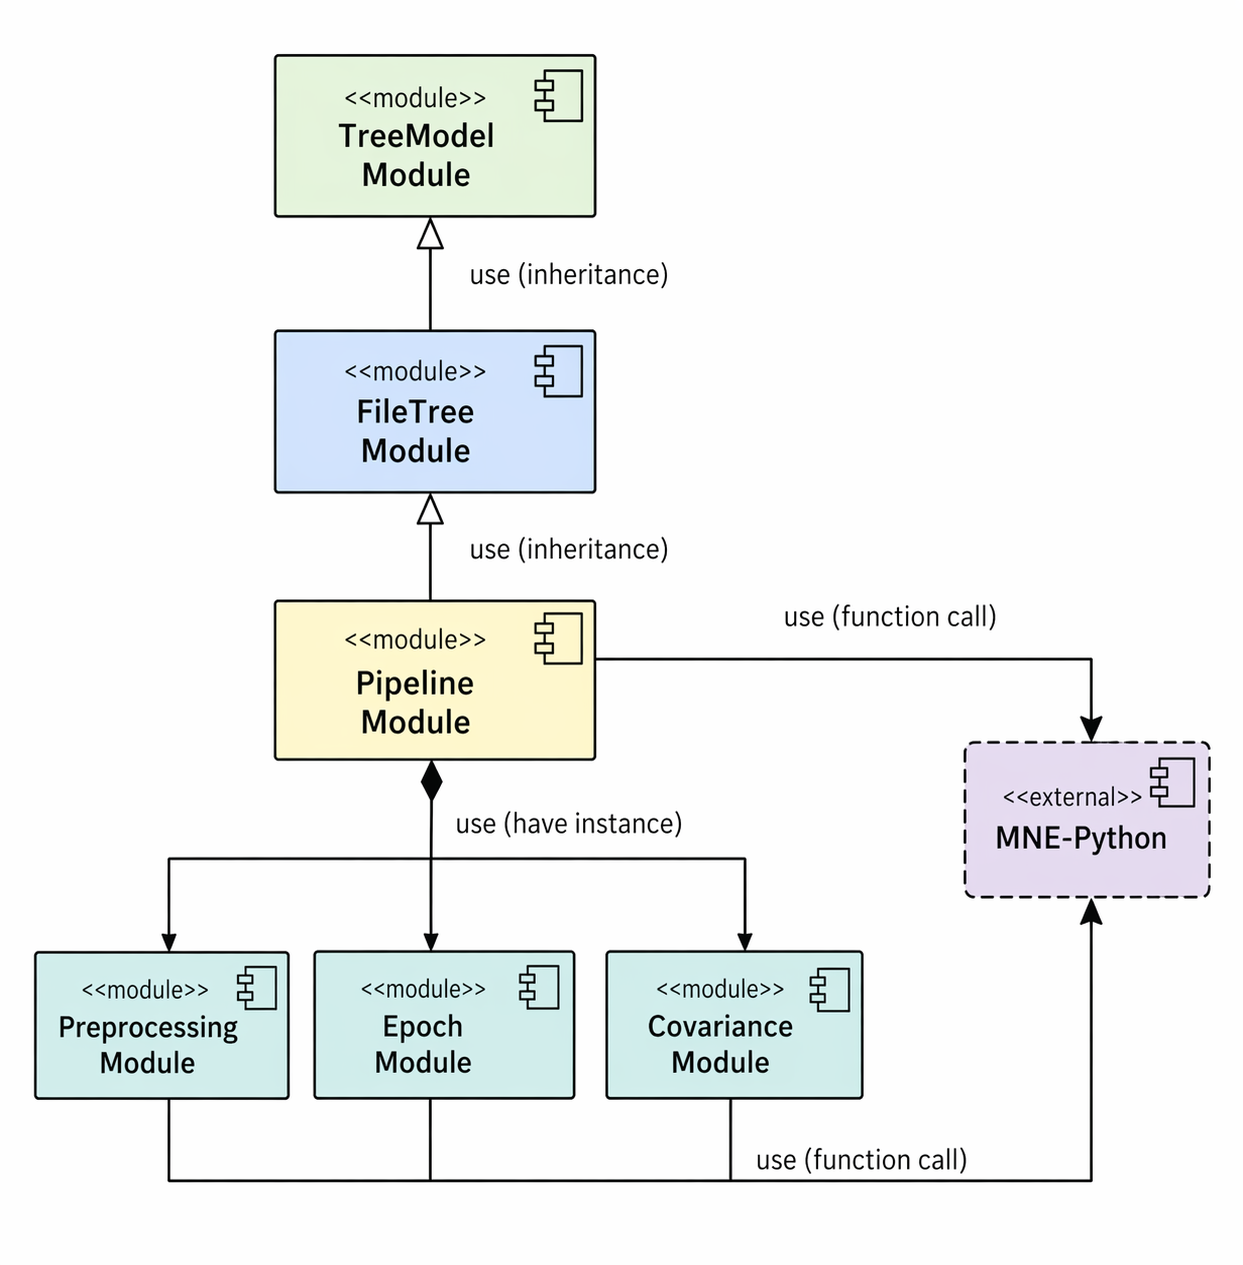
\includegraphics[width=0.7\textwidth]{use_hierarchy_uml.png}
\caption{Use hierarchy among modules}
\label{FigUH}
\end{figure}

%\section*{References}








% 10 User Interfaces
\section{User Interfaces}


\progname{} is a tool for command line or Jupyter Notebook usage. Pipeline Module (M1) serves as user interface.








% 11 Design of Communication Protocols
\section{Design of Communication Protocols}

NA








% 12 Database Design
\section{Database Design}


NA








% 13 Timeline
\section{Timeline}


Timeline is managed in \url{https://github.com/orgs/Eelbrain/projects/3}.








\bibliographystyle {plainnat}
\bibliography{../../../refs/References}


\newpage{}


\end{document}